\part{Results \& Discussion}
\section{Results}
For the default initial parameters\footnote{8 people, sea level pressure, 50\% humidity, $T_a=T_o=20$\degree C}, the results for crop production and energy consumption are shown below (Figures \ref{fig:results_crop} and \ref{fig:results_energy}). 

Crop production was cyclical at roughly 90 days between harvests. The area required for crop growth was 106 m$^2$/person and an initial supply of 54 kg/person of grain was needed to meet demand until the first harvest.

Energy usage for BioSim was distributed mainly to crop growth (lighting), which accounted for 79.6\% of total energy usage during daylight hours, while the next highest energy user was evaporation of concentrated RO brine (19.7\%). The remaining energy demands (living area lighting, RO pump, and UV disinfection) contributed only 0.70\% of daylight energy requirements.

Treatment of wastewater was accomplished with minimal energy and area requirements. Total treatment area accounted for less than 2\% of total area with the constructed wetlands requiring the most area (2.1 m$^2$/person). The sedimentation basin was used to remove particles over 100 $\mu$m while the constructed wetland removed nearly 100\% of remaining TSS using a 70 mm day$^{-1}$ loading rate. Further, head loss in the wetland was found to be near 0 using the Ergun equation.
\begin{figure}[h]
    \centering
    \begin{subfigure}[h]{.47\textwidth}
        \centering
        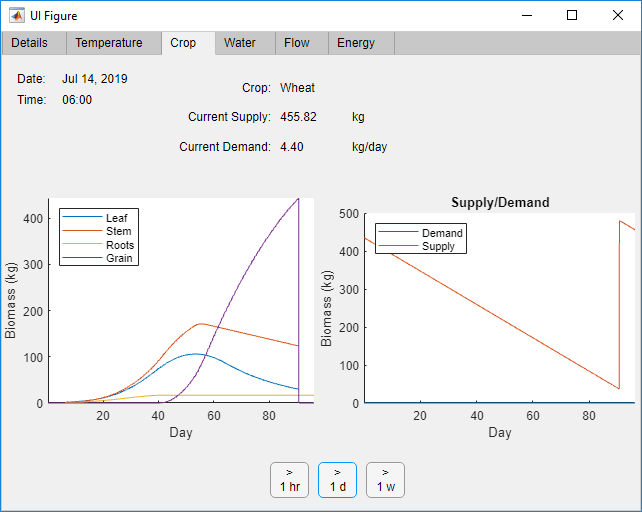
\includegraphics[width=\textwidth]{results_crop}
        \caption{Crop Growth results}
        \label{fig:results_crop}
    \end{subfigure}
    \hfill
    \begin{subfigure}[h]{.47\textwidth}
        \centering
        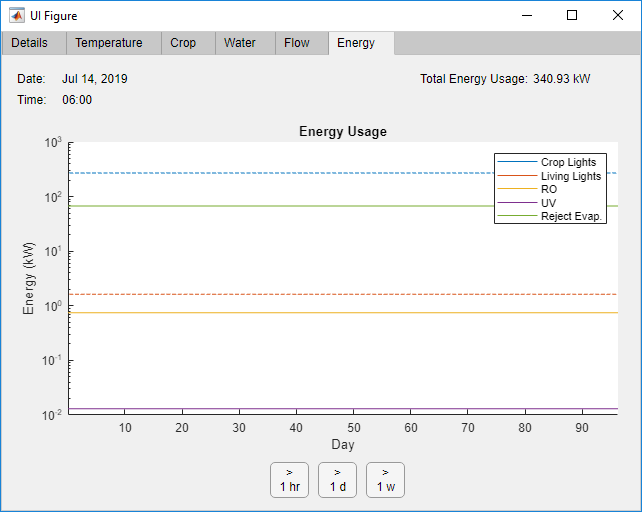
\includegraphics[width=\textwidth]{results_energy}
        \caption{Energy Consumption results}
        \label{fig:results_energy}
    \end{subfigure}
\end{figure}

\section{Discussion}
While the results provide a meaningful glimpse into the construction of such an environment, there are many questions which remain unanswered due to the difficulty in modeling many of these systems, and a larger question of what good a model of this nature could serve in a real-world situation. 

Regarding the first set of questions, the crop growth system stands out as a difficult system to model. The equations which govern crop development and partitioning of biomass are dependent on several factors and while there are many rigorous models, the model chosen, albeit simple, requires a number of empirical parameters. Empirical data used in this study came from the investigation of rice crops in Asia \cite{RICEPEST} and it is reasonable to wonder if there is enough parallel between rice and wheat crops that the parameters controlling the partitioning of biomass in one can be used in the other. It would be interesting to compare these results to those of a more complete model such as CERES-Wheat, part of DSSAT (\url{https://apps.agapps.org/ide/serial/}), which was used in Biosphere 2 to model wheat growth to within 10\% accuracy \cite{biosphere_wheat}. 

There is also a question regarding the completeness of a diet which is 100\% wheat. The crop was chosen because of the ease of access to relevant information and was only configured to provide the required 2000 calories per day. But there are several limitations in consuming just one crop and especially one that is not so nutritionally robust. Ideally, as was done in Biosphere 2, multiple crops of different varieties and nutritional compositions were grown which provided the required calories as well as vitamins and minerals, with supplements integrated as needed \cite{biosphere_diet}.

Another variable which could use further exploration is the area configured for crop growth. Currently, the area is configured to minimize the amount of storage necessary. In a real-life situation, there would be a trade-off between storage of the crop and the amount of area dedicated to growing crops. Alternative means of food production should thus be explored as well. Other techniques, such as hydroponics or aquaponics, may provide a reduction in the amount of space required without sacrificing total crop/calorie production. In the case of aquaponics, which is a hydroponics system combined with an aquaculture system, an additional source of protein can be grown alongside crops which is otherwise difficult to find in plant-based sources.

Biosphere 2's agriculture module provided 7 people a year-round nutritionally dense diet with about 2000 m$^3$ of area and hosted a diverse ecology of insects and animals \cite{biosphere_agriculture}. If a human habitat were to be constructed on Mars, a bigger discussion over the cost and feasibility of such a large area per person would need to take place since the resources necessary to build it will either need to be made on Mars or shipped from Earth. Concrete, for example, can likely be redesigned for Mars's unique soil chemistry and not have to be transported from Earth \cite{mars_concrete}, however the same soil will require fertilizers in order to grow crops \cite{mars_soil_crops}.

Carbon and nitrogen cycles were not modeled in this experiment. One of the larger issues in real-life experiments of this type, like Biosphere 2, was controlling high CO$_2$ and maintaining adequate oxygen levels. The authors state:
\begin{quote}
    The studies revealed that the agricultural biome was the greatest contributor of CO$_2$, due to carbon rich soil, to the atmosphere and the greatest consumer of atmospheric O$_2$, which was then locked up primarily in the massive concrete structural elements of the facility. This one way flow of O$_2$ bound by CO$_2$ into the concrete as carbonates and the low leak rates, resulted in a potentially life-threatening circumstance for the Biospherians that ultimately required the injection of O$_2$ \cite{biosphere_intro}.
\end{quote}

A fully-developed extension of BioSim would likely be necessary in predicting many of these factors and determining feasibility and cost estimates. Projects like Bios-3 and Biosphere 2 uncovered some surprising aspects of these constructed environments and contributed to the list of questions which must be answered before settling on the Moon or Mars. Still, it seems, there is a lot of work that remains before an extraterrestrial human settlement is a foregone conclusion.